\subsubsection{Subsystem Overview}
The platform management board manages all I/O required by the computing platform: interfacing with the camera, programmable logic board (hosting the machine learning implementation), and base station. A separate system is used for the multirotor's flight control.

A decomposition of the system is seen in Figure \ref{pcdiag}.

\begin{figure}[H]
\centering
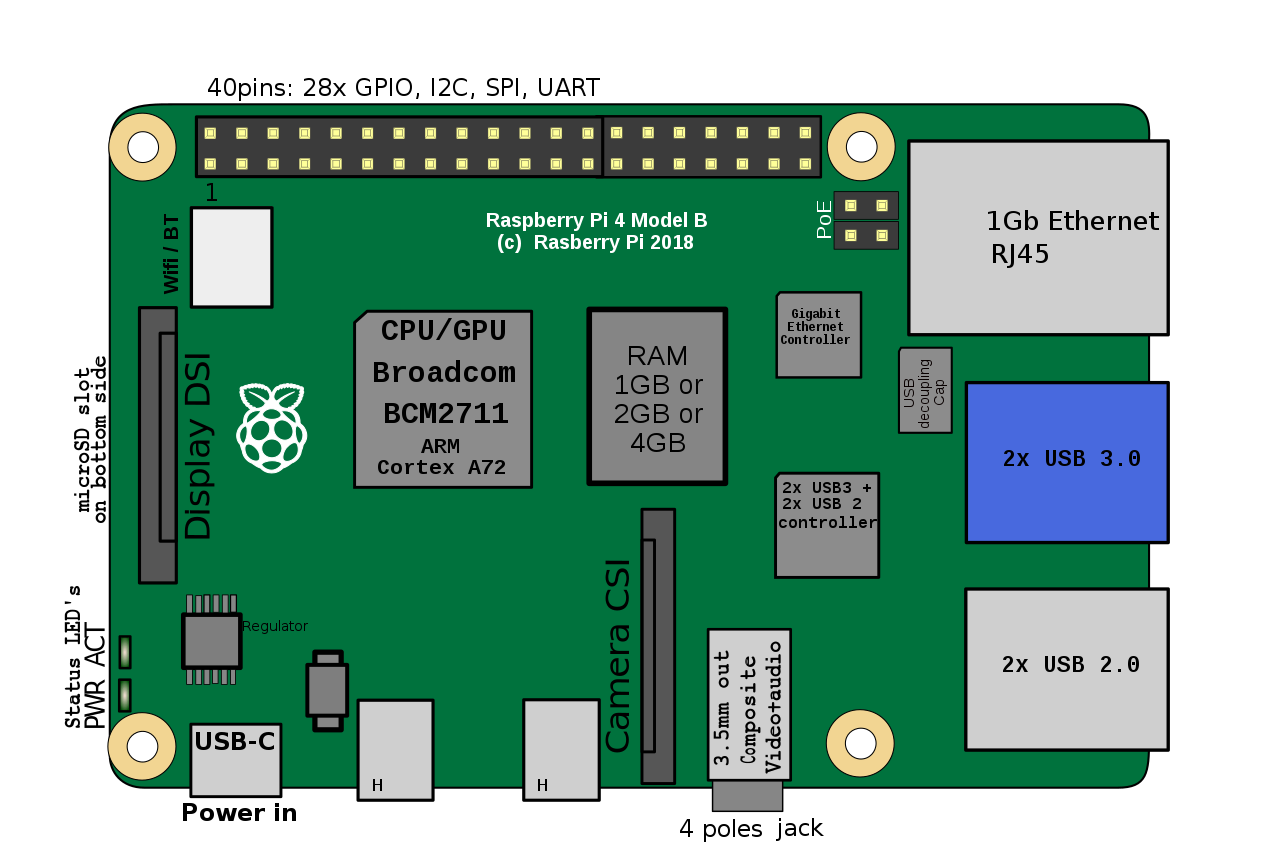
\includegraphics[width=10cm]{img/RaspberryPi_Model_4B.png}
\caption[Layout of Connectors and Main ICs on Raspberry Pi 4]{Layout of Connectors and Main ICs on Raspberry Pi 4\cite{rpidiag}}
\label{rpi}
\end{figure}

\subsubsection{Device Selection}

The selected device to implement the platform management system is the Raspberry Pi 4. As seen in Figure \ref{rpi}, the Raspberry Pi 4 is a small single-board computer that hosts a quad-core ARM Cortex A72 CPU, a CSI camera interface, 40 serial pins, Wi-Fi/Bluetooth, and a gigabit Ethernet port. We chose the Raspberry Pi 4 over other single-computer platforms (including Arduino, Beagleboard, and Orange Pi) because the Raspberry Pi 4:

\begin{itemize}
\item is relatively inexpensive (CAN\$45 in November 2019) compared to similarly outfitted single-board computers,
\item has a large support community and a wealth of driver/library support,
\item supports a wide range of high throughput I/O standards (USB/WiFi/Ethernet/Serial, \textbf{C.EX.3}),
\item provides an industry-standard camera interface (\textbf{C.EX.5}),
\item supports extensible non-volatile storage (\textbf{F.CP.4}),
\item and is presumed to have a cross-compatible successor (the Raspberry Pi 5) -- therefore future-proofing the PMB segment.
\end{itemize} 

\subsubsection{Data Flow}
\label{pmb_dataflow}
The Platform Management Board manages the data flow as follows:
\begin{enumerate}
\item The CSI interface is utilized to acquire a video frame ($640px \times 480px$) from the camera
\item The PMB performs frame manipulation/correction if required by the specific machine learning use-case. The YOLOv2 accelerator (described in Section \ref{ml_accel}) necessitates images sent to the Zedboard to be letterboxed to $416px \times 416px$ to adhere to ML IP block restrictions.
\item The letterboxed frame is decomposed and transmitted over Ethernet to the programmable logic board (which performs the machine learning)
\begin{enumerate}
\item While waiting for the machine learning results, the PMB sends full-resolution ($640px \times 480px$) frames to the Base Station --- allowing for higher ``background" framerate rather than tying framerate to ML results.
\end{enumerate}
\item The PLB returns the machine learning results to the PMB via Ethernet
\item The PMB's WiFi modem transmits full-resolution video, ML results, and system status information to the base station
\item Results and video are additionally stored locally on non-volatile storage for post-flight analysis\footnote{This functionality was foregone due to COVID-19 imposed time constraints. There are no functional restrictions for this to be accomplished, however without a comprehensive interface to facilitate easy retrieval of footage (which would require significant development effort), it is easier for the client to record the web-app directly.}
\end{enumerate}

On the PMB broad there are two programs, a C++ program and a Python client, that are running while in operation.The C++ program handles image capture and data transmission with the PLB. The Python program handles the data transmission with the base station, that is, it sends the image data and machine learning result to the base station and receives the control message from the base station. The reason behind using two separate programs is that the communication between the PMB and the base station is using Socket.IO library. Socket.IO is a communication library that uses TCP as its transport layer protocol. The PMB's operating system has a much better support for the Python version of the Socket.IO library than the C++ version Socket.IO library.

All operations are managed by the ARM Cortex A72 chip running a headless version of the Raspbian operating system. 

With the provided ML accelerator implementation (described in Section \ref{plb_sec}), the delay visible to the PMB between ML request issuance and reply (steps 3 and 4) is approximately two seconds. Excess speed in the motions of the multirotor and/or the detected objects will result in the detection bounding boxes \textit{trailing} the objects in the live video by approximately two seconds. To resolve this issue, the user may configure the system to operate on a ``tape-delay" basis. In this configuration, the live video is delayed by an equal amount of time as it takes for the ML results to be generated. While this provides results which are better matched to the video displayed to the user, the added video delay may be disorienting if the video feed is used for flying the multirotor. The user should not rely on the this video footage to attempt to control the multirotor.

\subsubsection{Use of Multiple Computing Boards}
The presence of on-board Wi-Fi and camera interfaces is the primary driving factor towards adopting a dual-board (PMB and PLB) solution. While a uni-board solution is possible, the development effort and cost of the computing platform would be considerably higher. Most programmable logic boards (including our chosen board, the Zedboard) require external expansion devices to interface with peripherals such as WiFi adapters/cameras. These expansion devices, which connect to the programmable logic board via a serial connection, have poorly documented drivers and are of considerable expense -- ranging from US\$25 for a basic WiFi module\cite{digiwifi} to US\$200 for a compatible camera interface card\cite{digipmod}. External expansion devices also require considerable glue logic on the programmable logic board, potentially risking non-compliance with constraint \textbf{C.EX.2}.

An additional consideration in selecting the two-board design regards platform extensibility --- the client may desire to increase the programmable logic capabilities of the computing platform in the future, requiring a board swap. If a single-board solution is implemented, the client would be required to migrate \textit{all} hardware/software to the larger board, requiring them to devote considerable effort to debug driver issues. Additionally, external expansion devices are not necessarily compatible with all PLBs -- adding constraints to the client's board selection or requiring the purchase of new interface cards. By offloading the interfacing work to a distinct \textit{platform management} board, the client can easily replace the PLB without considerable redevelopment (fulfilling constraint \textbf{C.EX.4}). 

To emphasize, the use of multiple computing boards is a design decision derived from the current budgetary constraint to use \textit{off-the-shelf} components in the development of this device. Upon the completion of new hardware-accelerated machine learning implementations, the client may wish to integrate the capabilities of both boards into a single (custom ASIC) platform (at a considerable expense). 

\subsubsection{Interface with Programmable Logic Board}

To interface with the PLB, video frames are sent via a bi-directional Ethernet connection (TCP/IP socket). TCP/IP over Ethernet was selected in lieu of serial solutions as:
\begin{itemize}
\item Ethernet is equally as ubiquitous on modern programmable logic boards
\item Ethernet has higher maximum throughput on modern platforms (on the Zedboard, 1 Gbps on Ethernet vs. 400 Kbps on serial)
\item Ethernet has more robust error control coding schemes (such as implicit forward error correction\cite{mclaughlin_warland}) compared to serial, leading to more reliable data transfer
\end{itemize} 

The selection of Ethernet over serial precludes the use of the \textit{Zero W} variant of the Raspberry Pi, as the Zero W does not provide Ethernet support. 

Utilizing gigabit Ethernet also allows for the transmission of uncompressed (raw-RGB) images to the PLB with minimal-to-no additional latency. While both platforms are capable of doing such image manipulations on-the-fly, the compression/decompression imposes additional overhead on the critical path (particularly when decompressing images on the slower PLB) which can be avoided through this approach. 

\subsubsection{Interface with Base Station}

As detailed in Section \ref{pmb_dataflow}, video, ML results, and system status information is broadcast to the Base Station using the on-board WiFi modem. WiFi was utilized over other competing wireless standards (such as Bluetooth and Zigbee) due to its high throughput, excellent range, and ubiquitous market share across possible client devices.

Several WiFi networking structures were examined when determining which device would act as the communications 'host' (i.e., whether the Base Station or PMB would act as as the server). Through in-field experiments it was determined that the optimal configuration consists of the PMB acting as the \textit{client} connecting to a dedicated networking card acting as the \textit{server} at the Base Station. This is in contrast to hosting a wireless network directly from the PMB, which is not the intended use of the on-board WiFi modem (with sub par firmware support and insufficient antenna gain resulting in poorer signal reliability). 

Additional operational range could be achieved through the purchase of a dedicated, Raspbian-compatible WiFi dongle. The integration of such a dongle would require no significant change to the system (automatically superseding the current modem upon installation). Such an installation, however, would evidently need to be juxtaposed with the the additional weight considerations instilled by the dongle, potentially impacting flight duration/quality.
